% !TeX program = xelatex
\documentclass[a4paper,10pt]{article}

% ============================================================================
% សន្លឹកកិច្ចការសិស្ស ស-ខ្មៅ (Student Fill-In Worksheet — No-LCD Classroom)
% មេរៀនទី១៧ (១៧.១.២)៖ ផ្ទៃក្រឡាខាងនិងផ្ទៃក្រឡាទាំងអស់នៃពីរ៉ាមីត (ត្រូវគ្នា ១០០% នឹង LS_Plan_PYR_SA.tex)
% ============================================================================
\usepackage[a4paper, left=0.95cm, right=0.95cm, top=0.75cm, bottom=0.90cm, footskip=0.48cm]{geometry}
\usepackage{amsmath}
\usepackage{unicode-math}
\usepackage{fontspec}
\usepackage{array, colortbl}
\usepackage[table]{xcolor}
\usepackage{enumitem}
\usepackage{pifont}
\usepackage{fancyhdr}
\usepackage{lastpage}
\usepackage{tikz}
\usepackage[most]{tcolorbox}
\usetikzlibrary{calc, arrows.meta, angles, quotes, patterns, decorations.markings, babel}

\makeatletter
\let\@expl@@@mark@update@singlecol@structures@@\relax
\makeatother

\providecommand{\NGSFindFonts}{%
  \IfFileExists{C:/Windows/Fonts/cambria.ttc}{%
    \def\NGSSysPath{C:/Windows/Fonts/}%
    \def\NGSUserPath{C:/Users/KIT/AppData/Local/Microsoft/Windows/Fonts/}%
  }{%
    \IfFileExists{./fonts/KhmerOSsiemreap.ttf}{\def\NGSSysPath{./fonts/}\def\NGSUserPath{./fonts/}}{%
    \IfFileExists{../fonts/KhmerOSsiemreap.ttf}{\def\NGSSysPath{../fonts/}\def\NGSUserPath{../fonts/}}{%
    \IfFileExists{../../fonts/KhmerOSsiemreap.ttf}{\def\NGSSysPath{../../fonts/}\def\NGSUserPath{../../fonts/}}{%
    \IfFileExists{../../../fonts/KhmerOSsiemreap.ttf}{\def\NGSSysPath{../../../fonts/}\def\NGSUserPath{../../../fonts/}}{%
    \IfFileExists{../../../../fonts/KhmerOSsiemreap.ttf}{\def\NGSSysPath{../../../../fonts/}\def\NGSUserPath{../../../../fonts/}}{%
    \IfFileExists{../../../../../fonts/KhmerOSsiemreap.ttf}{\def\NGSSysPath{../../../../../fonts/}\def\NGSUserPath{../../../../../fonts/}}{%
    \IfFileExists{../../../../../../fonts/KhmerOSsiemreap.ttf}{\def\NGSSysPath{../../../../../../fonts/}\def\NGSUserPath{../../../../../../fonts/}}{%
      \def\NGSSysPath{../../../../../../../fonts/}\def\NGSUserPath{../../../../../../../fonts/}%
    }}}}}}}%
  }%
}
\NGSFindFonts

\setmathfont[Path={\NGSSysPath}, FontIndex=1, Scale=1.02]{cambria.ttc}
\defaultfontfeatures{Ligatures=TeX}

\setmainfont[
  Path={\NGSUserPath},
  Extension=.ttf,
  Script=Khmer,
  BoldFont={KhmerOSsiemreap},
  BoldFeatures={FakeBold=1.8},
  ItalicFont={KhmerOSsiemreap},
  ItalicFeatures={FakeSlant=0.25},
  BoldItalicFont={KhmerOSsiemreap},
  BoldItalicFeatures={FakeBold=1.8, FakeSlant=0.25}
]{KhmerOSsiemreap}

\newfontfamily\muol[Path={\NGSUserPath}, Extension=.ttf, Script=Khmer]{KhmerOSmuollight}
\newfontfamily\TimesEn[Path={\NGSSysPath}, Extension=.ttf, BoldFont={timesbd}, ItalicFont={timesi}, BoldItalicFont={timesbi}]{times}

\XeTeXlinebreaklocale "km"
\XeTeXlinebreakskip = 0pt plus 1pt minus 0.1pt

\definecolor{panelgray}{gray}{0.93}
\definecolor{headgray}{gray}{0.85}

\pagestyle{fancy}
\fancyhf{}
\renewcommand{\headrulewidth}{0pt}
\fancyfoot[L]{\fontsize{8pt}{10pt}\selectfont អនុវិទ្យាល័យព្រះក្រសាំង \en{---} គណិតវិទ្យា ថ្នាក់ទី៨ \en{|} មេរៀនទី១៧ (១៧.១ ផ្ទៃក្រឡាខាងនិងផ្ទៃក្រឡាទាំងអស់នៃពីរ៉ាមីត)}
\fancyfoot[R]{\fontsize{8.2pt}{10pt}\selectfont ទំព័រ \en{\thepage\ / \pageref{LastPage}}}

\setlength{\parindent}{0pt}
\setlength{\parskip}{0pt}
\setlength{\tabcolsep}{4pt}

\newcommand{\en}[1]{{\TimesEn #1}}
\newcommand{\enbf}[1]{{\TimesEn\textbf{#1}}}
\newcommand{\unit}[1]{\,\text{\en{#1}}}
\newcommand{\cnum}[1]{\mbox{\fontsize{10pt}{12pt}\selectfont\ding{\numexpr181+#1\relax}}}
\newcommand{\chkbox}{\tikz[baseline=-0.15ex]\draw[black, line width=0.85pt] (0,0) rectangle (0.25cm,0.25cm);}
\newcommand{\blank}[1]{\makebox[#1]{\dotfill}}
\newcommand{\tri}[1]{\ensuremath{\triangle #1}}

\newcommand{\rightbox}[4][0.18]{%
  \draw[black, line width=0.8pt]
    ($(#3)!#1!(#2)$) -- ($($(#3)!#1!(#2)$)+($(#3)!#1!(#4)$)-(#3)$) -- ($(#3)!#1!(#4)$);
}

\newcommand{\secbar}[2]{%
  \vspace{3pt}%
  \begin{tcolorbox}[
    enhanced, sharp corners, colback=headgray, colframe=black,
    boxrule=0.9pt, boxsep=1pt, top=2.5pt, bottom=2.5pt, left=6pt, right=6pt,
    after skip=3pt
  ]
    {\muol\fontsize{9.2pt}{13.5pt}\selectfont #1}\hfill{\fontsize{8.3pt}{11.5pt}\selectfont\textbf{#2}}
  \end{tcolorbox}%
}

\newcolumntype{L}[1]{>{\raggedright\arraybackslash}p{#1}}
\newcolumntype{C}[1]{>{\centering\arraybackslash}p{#1}}

\begin{document}
\fontsize{9.4pt}{13.8pt}\selectfont

% ============================================================================
% ទំព័រទី ១៖ ក្បាលសន្លឹកកិច្ចការ + E1 + E2 (បែងចែកធាតុ ៣ & ស្ពានពីតាករ) + E3 (និយមន័យ & រូបមន្ត)
% ============================================================================
\begin{tcolorbox}[
  enhanced, sharp corners, colback=white, colframe=black,
  boxrule=1.1pt, boxsep=2.5pt, top=5.5pt, bottom=5.5pt, left=6pt, right=6pt, after skip=6.5pt
]
  \begin{center}
    {\muol\fontsize{10pt}{14.5pt}\selectfont សន្លឹកកិច្ចការសិស្ស \enbf{---} គណិតវិទ្យា ថ្នាក់ទី៨ \enbf{(}១៧\enbf{.}១ ផ្ទៃក្រឡាខាងនិងផ្ទៃក្រឡាទាំងអស់នៃពីរ៉ាមីត\enbf{)}}\\[3.5pt]
    {\fontsize{8.8pt}{12pt}\selectfont
    ឈ្មោះសិស្ស / ដៃគូ៖ \blank{6.2cm} \hspace{0.2cm}
    ថ្នាក់៖ \blank{1.4cm} \hspace{0.2cm}
    ក្រុម៖ \blank{1.2cm} \hspace{0.2cm}
    កាលបរិច្ឆេទ៖ \blank{2.8cm}}
  \end{center}
\end{tcolorbox}

% --- E1 Engage ---
\begin{tcolorbox}[
  enhanced, sharp corners, colback=panelgray, colframe=black,
  boxrule=0.8pt, boxsep=2.5pt, top=5.5pt, bottom=5.5pt, left=6pt, right=6pt, after skip=6.5pt
]
  \textbf{បេសកកម្មទី១ (\en{E1 - Engage})៖ ដំបូលខ្ចូសរាងពីរ៉ាមីតចតុមុខនិយ័ត — ទ្រនុងខាង ទល់នឹង អាប៉ូតែម!}\\[2pt]
  ដំបូលខ្ចូសមួយមានរាងជាពីរ៉ាមីតចតុមុខនិយ័ត មានជ្រុងបាតការេ $AB=12$ និងផ្លានជ្រុង (ទ្រនុងខាង) $SA=10$ ។ \textbf{ជាង ក} គណនាផ្ទៃត្រីកោណមុខខាងមួយស្មើ $\frac{1}{2}\times 12\times 10 = 60$ ឯ \textbf{ជាង ខ} ថាខុស ព្រោះ $10$ ជាទ្រនុងខាង មិនមែនជាកម្ពស់ត្រីកោណមុខខាង ($SH\perp AB$) ទេ!\\[2pt]
  \ding{226}\ ចូរទស្សន៍ទាយជាដៃគូ៖ \;\chkbox\ ជាង ក ត្រឹមត្រូវ \hspace{0.5cm} \chkbox\ ជាង ខ ត្រឹមត្រូវ \hspace{0.5cm} \chkbox\ ទាំងពីរស្មើគ្នា
\end{tcolorbox}

% --- E2 Explore Part A: 3-Segment Distinction & Star Net ---
\secbar{ផ្នែកទី១ \enbf{(}ក\enbf{)} ៖ បែងចែកធាតុទាំង ៣ នៃពីរ៉ាមីត និងគំនូសលាតផ្កាយ \enbf{2D (E2 - Explore)}}{ការងារជាដៃគូ \en{5 min}}

\noindent
\begin{minipage}[c]{9.0cm}
  \centering
  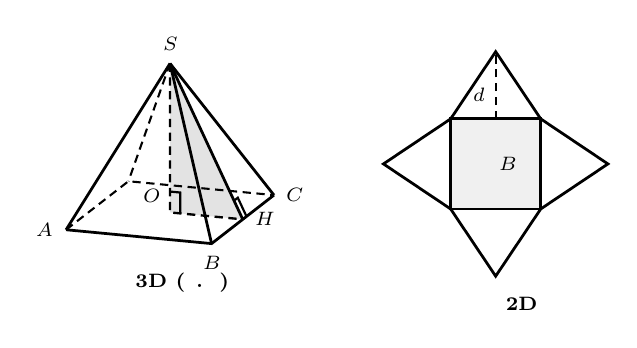
\begin{tikzpicture}[scale=0.88, every node/.style={font=\scriptsize, text=black}]
    % រូបឆ្វេង៖ ពីរ៉ាមីតចតុមុខនិយ័ត និងត្រីកោណកែងខាងក្នុង
    \begin{scope}[shift={(-2.55,0)}]
      \coordinate (A) at (-1.50,-0.95);
      \coordinate (B) at (0.60,-1.15);
      \coordinate (C) at (1.50,-0.45);
      \coordinate (D) at (-0.60,-0.25);
      \coordinate (O) at (0.0,-0.70);
      \coordinate (S) at (0.0,1.45);
      \coordinate (H) at (1.05,-0.80);
      \fill[gray!22] (S) -- (O) -- (H) -- cycle;
      \draw[black, line width=1.0pt] (A) -- (B) -- (C);
      \draw[black, line width=0.75pt, densely dashed] (A) -- (D) -- (C);
      \draw[black, line width=1.0pt] (S) -- (A) (S) -- (B) (S) -- (C);
      \draw[black, line width=0.75pt, densely dashed] (S) -- (D);
      \draw[black, line width=1.0pt] (S) -- (H);
      \draw[black, line width=0.85pt, densely dashed] (S) -- (O) -- (H);
      \rightbox[0.14]{S}{O}{H}
      \rightbox[0.12]{S}{H}{C}
      \node[above=1pt] at (S) {$S$};
      \node[above left=0pt] at (O) {$O$};
      \node[right=1pt] at (H) {$H$};
      \node[left=1pt] at (A) {$A$};
      \node[below=1pt] at (B) {$B$};
      \node[right=1pt] at (C) {$C$};
      \node at (0.0,-1.72) {\textbf{រូប \enbf{3D} (ទំ.២១៨)}};
    \end{scope}

    % រូបស្ដាំ៖ គំនូសលាតផ្កាយ 2D
    \begin{scope}[shift={(2.15,0)}]
      \draw[black, line width=1.0pt, fill=gray!12] (-0.65,-0.65) rectangle (0.65,0.65);
      \draw[black, line width=1.0pt] (-0.65,0.65) -- (0,1.62) -- (0.65,0.65);
      \draw[black, line width=1.0pt] (-0.65,-0.65) -- (0,-1.62) -- (0.65,-0.65);
      \draw[black, line width=1.0pt] (-0.65,-0.65) -- (-1.62,0) -- (-0.65,0.65);
      \draw[black, line width=1.0pt] (0.65,-0.65) -- (1.62,0) -- (0.65,0.65);
      \draw[black, line width=0.8pt, densely dashed] (0,0.65) -- (0,1.62);
      \node at (0,0) {\textbf{បាត $B$}};
      \node[left=0.5pt] at (0,1.00) {$d$};
      \node at (0.0,-2.02) {\textbf{លាតផ្កាយ \enbf{2D}}};
    \end{scope}
  \end{tikzpicture}
\end{minipage}%
\hfill
\begin{minipage}[c]{9.6cm}\raggedright
  \textbf{បំពេញឈ្មោះធាតុនៃពីរ៉ាមីតតាមសៀវភៅទំព័រ ២១៨៖}\\[6.5pt]
  $1.$ ពីរ៉ាមីតមាន \textbf{បាត} ចំនួន \blank{0.9cm} គត់ ហើយមុខខាងទាំងអស់ជារូប \blank{2.3cm} ដែលប្រសព្វគ្នាត្រង់ \textbf{កំពូល} $S$ ។\\[6pt]
  $2.$ ជ្រើសរើសពាក្យ \textbf{(កម្ពស់ / អាប៉ូតែម / ជនេត្រ ឬទ្រនុងខាង)}៖\\[4pt]
  \hspace*{0.2cm}$\bullet$ អង្កត់ $SO\perp$ ប្លង់បាតត្រង់ផ្ចិត $O$ ហៅថា៖ \textbf{\blank{2.6cm}}\\[4.5pt]
  \hspace*{0.2cm}$\bullet$ អង្កត់ $SH\perp BC$ (កម្ពស់ត្រីកោណមុខខាង) ហៅថា៖ \textbf{\blank{2.5cm}}\\[4.5pt]
  \hspace*{0.2cm}$\bullet$ អង្កត់ $SA, SB, SC$ ភ្ជាប់កំពូលទៅកំពូលបាតហៅថា៖ \textbf{\blank{2.4cm}}
\end{minipage}

\vspace{14pt}
% --- E2 Explore Part B: Pythagorean Bridge on Worked Example 1 ---
\secbar{ផ្នែកទី១ \enbf{(}ខ\enbf{)} ៖ ស្ពានពីតាកររកអាប៉ូតែម \enbf{---} លំហាត់គំរូទី \enbf{1 (}ទំព័រ ២១៩\enbf{)}}{ការងារជាដៃគូ \en{6 min}}

\noindent
\begin{minipage}[c]{6.2cm}
  \centering
  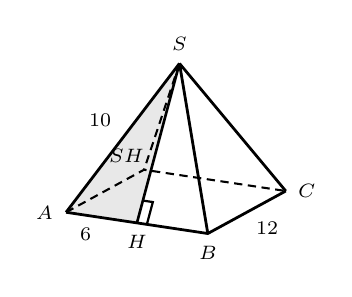
\begin{tikzpicture}[scale=0.90, every node/.style={font=\scriptsize, text=black}]
    \coordinate (A) at (-1.55,-0.65);
    \coordinate (B) at (0.45,-0.95);
    \coordinate (C) at (1.55,-0.35);
    \coordinate (D) at (-0.45,-0.05);
    \coordinate (S) at (0.05,1.45);
    \coordinate (H) at ($0.5*(A)+0.5*(B)$);
    \fill[gray!18] (S) -- (A) -- (H) -- cycle;
    \draw[black, line width=1.0pt] (A) -- (B) -- (C) (S) -- (A) (S) -- (B) (S) -- (C);
    \draw[black, line width=0.75pt, densely dashed] (A) -- (D) -- (C) (S) -- (D);
    \draw[black, line width=0.95pt] (S) -- (H);
    \rightbox[0.14]{S}{H}{B}
    \node[above=1pt] at (S) {$S$};
    \node[left=1pt] at (A) {$A$};
    \node[below=1pt] at (B) {$B$};
    \node[right=1pt] at (C) {$C$};
    \node[below=1pt] at (H) {$H$};
    \node[above left=0.5pt] at ($0.5*(S)+0.5*(A)$) {$10$};
    \node[below left=0pt] at ($0.5*(A)+0.5*(H)$) {$6$};
    \node[below right=0pt] at ($0.5*(B)+0.5*(C)$) {$12$};
    \node[left=1pt] at ($0.42*(S)+0.58*(H)$) {$SH$};
  \end{tikzpicture}
\end{minipage}%
\hfill
\begin{minipage}[c]{12.4cm}\raggedright
  \textbf{លំហាត់គំរូទី \en{1} (ទំ.២១៩)៖} ពីរ៉ាមីតចតុមុខនិយ័តមានជ្រុងបាតការេ $12$ និងទ្រនុងខាង $SA=10$ ។\\[6.5pt]
  $1.$ $H$ ជាចំណុចកណ្ដាលជ្រុង $AB \Rightarrow AH = \dfrac{12}{2} = \blank{0.9cm}$ ។ តាមទ្រឹស្ដីបទពីតាករក្នុង $\tri{SAH}$ កែងត្រង់ $H$៖\\[5pt]
  \hspace*{0.3cm}$AH^2 + SH^2 = SA^2 \Rightarrow SH^2 = 10^2 - (\blank{0.7cm})^2 = 100 - \blank{0.9cm} = \blank{0.9cm} \Rightarrow SH = \blank{1.0cm}$ ។\\[6.5pt]
  $2.$ \textbf{ក. ផ្ទៃក្រឡាខាង ($S_l$)៖} $S_l = 4 \times \dfrac{1}{2} \times (\blank{0.8cm}\times 12) = \blank{1.4cm}$ ឯកតាផ្ទៃ ។\\[6.5pt]
  $3.$ \textbf{ខ. ផ្ទៃក្រឡាទាំងអស់ ($S_t$)៖} $S_t = S_l + B = \blank{1.2cm} + (12\times 12) = \blank{1.2cm} + \blank{1.1cm} = \blank{1.4cm}$ ឯកតាផ្ទៃ ។
\end{minipage}

\vspace{14pt}
% --- E3 Explain: Definitions & Formula Summary ---
\secbar{ផ្នែកទី២ ៖ និយមន័យពីរ៉ាមីតនិយ័ត និងរូបមន្តផ្ទៃក្រឡាពីរ៉ាមីត \enbf{(E3 - Explain)}}{សង្ខេបរួមគ្នា \en{6 min}}

\begin{tcolorbox}[
  enhanced, sharp corners, colback=white, colframe=black,
  boxrule=0.9pt, boxsep=4pt, top=7.5pt, bottom=7.5pt, left=6pt, right=6pt
]
  $\bullet$ \textbf{ពីរ៉ាមីតនិយ័ត (ទំ.២១៨)៖} ជាពីរ៉ាមីតដែលមានបាតជា \textbf{\blank{2.8cm}} និងទ្រនុងខាងទាំងអស់ \textbf{\blank{1.8cm}} ។ មុខខាងទាំងអស់នៃពីរ៉ាមីតនិយ័តជា \textbf{\blank{3.4cm}} ។ \textit{(ប្រយ័ត្ន៖ បើបាតជាចតុកោណកែង $l\neq w$ នោះវាមិនមែនជាពីរ៉ាមីតនិយ័តទេ!)} \\[7.5pt]
  {\renewcommand{\arraystretch}{1.80}\footnotesize
  \begin{tabular}{|L{5.10cm}|L{5.65cm}|L{6.35cm}|}
    \hline
    \cellcolor{headgray}\textbf{បរិមាណផ្ទៃក្រឡានៃពីរ៉ាមីត} & \cellcolor{headgray}\textbf{រូបមន្តគណនា} & \cellcolor{headgray}\textbf{ចំណុចសម្គាល់សំខាន់} \\
    \hline
    $1.$ ផ្ទៃក្រឡាខាងពីរ៉ាមីតទូទៅ ($S_l$) & $S_l = \text{ផលបូកផ្ទៃត្រីកោណមុខខាងទាំងអស់}$ & ចំពោះបាតចតុកោណកែង ត្រូវរកអាប៉ូតែមទាំង ២ គូ! \\
    \hline
    $2.$ ផ្ទៃក្រឡាខាងពីរ៉ាមីតនិយ័ត ($S_l$) & $S_l = \dfrac{1}{2}\, \blank{0.9cm} \times \blank{0.9cm}$ & $P$ ជាបរិមាត្របាតនិយ័ត,\; $d$ ជាអាប៉ូតែមមុខខាង \\
    \hline
    $3.$ ផ្ទៃក្រឡាទាំងអស់នៃពីរ៉ាមីត ($S_t$) & $S_t = S_l + \blank{1.6cm}$ & បូកបាតតែ \textbf{១} គត់ (ខុសពីព្រីសដែលបូក $2B$!) \\
    \hline
  \end{tabular}}\\[7.5pt]
  $\bullet$ \textbf{ផ្ទៀងផ្ទាត់ការភាន់ច្រឡំ (ព្រីស ទល់នឹង ពីរ៉ាមីត)៖}
  \chkbox\ ព្រីសត្រង់៖ $S_l = P\cdot h,\; S_t = S_l + 2B$ \hspace{0.35cm}
  \chkbox\ ពីរ៉ាមីតនិយ័ត៖ $S_l = \frac{1}{2}P\cdot d,\; S_t = S_l + B$\\[6pt]
  $\bullet$ \textbf{ធនាគារហេតុផល៖}
  \cnum{1} ពីតាកររកអាប៉ូតែម $d$ \;\textbar\;
  \cnum{2} $S_l = \sum S_{\text{មុខខាង}}$ (ឬ $\frac{1}{2}Pd$) \;\textbar\;
  \cnum{3} $S_t = S_l + B$ \;\textbar\;
  \cnum{4} ដកមុខត្រួតគ្នាក្នុងសូលីតផ្សំ
\end{tcolorbox}

\newpage

% ============================================================================
% ទំព័រទី ២៖ E4 (លំហាត់គំរូទី 2 & ប្រតិបត្តិ ទំ.២១៩-២២០) + E5 (លំហាត់សូលីតផ្សំទី៤ & Exit Check) + កិច្ចការផ្ទះ
% ============================================================================

\secbar{ផ្នែកទី៣ ៖ អនុវត្តពីរ៉ាមីតបាតចតុកោណកែង \enbf{---} ទំព័រ ២១៩\enbf{--}២២០ \enbf{(E4 - Elaborate)}}{អនុវត្ត \en{10 min}}

\noindent
\begin{minipage}[t]{9.3cm}\vspace{0pt}
  \begin{tcolorbox}[
    enhanced, sharp corners, colback=white, colframe=black, equal height group=rowE4,
    boxrule=0.85pt, boxsep=3pt, top=5pt, bottom=5pt, left=5.5pt, right=5.5pt
  ]\raggedright
    \textbf{៣.ក លំហាត់គំរូទី \en{2} (ទំ.២១៩--២២០)៖ បាត $10\unit{cm}\times 18\unit{cm}$}\\
    បាតពីរ៉ាមីត $ABCDE$ មានរង្វាស់ $10\unit{cm}$ និង $18\unit{cm}$ កម្ពស់ $AF=12\unit{cm}$ ៖
    \begin{center}
      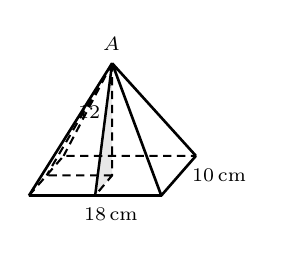
\begin{tikzpicture}[scale=0.80, every node/.style={font=\scriptsize, text=black}]
        \coordinate (C) at (-1.20,-0.85);
        \coordinate (D) at (0.90,-0.85);
        \coordinate (E) at (1.45,-0.22);
        \coordinate (B) at (-0.65,-0.22);
        \coordinate (F) at (0.12,-0.53);
        \coordinate (A) at (0.12,1.25);
        \coordinate (H) at (-0.15,-0.85);
        \coordinate (G) at (-0.92,-0.53);
        \fill[gray!18] (A) -- (F) -- (H) -- cycle;
        \draw[black, line width=0.95pt] (C) -- (D) -- (E) (A) -- (C) (A) -- (D) (A) -- (E);
        \draw[black, line width=0.75pt, densely dashed] (C) -- (B) -- (E) (A) -- (B) (A) -- (F) -- (H) (F) -- (G) (A) -- (G);
        \draw[black, line width=0.9pt] (A) -- (H);
        \node[above=1pt] at (A) {$A$};
        \node[below=1pt] at (0.10,-0.85) {$18\unit{cm}$};
        \node[right=1pt] at (1.20,-0.53) {$10\unit{cm}$};
        \node[left=0.5pt] at (0.12,0.48) {$12$};
      \end{tikzpicture}
    \end{center}
    $\bullet$ \textbf{ក.} ជាពីរ៉ាមីតនិយ័តឬទេ? \chkbox\ មែន \;\chkbox\ មិនមែន ព្រោះ \blank{2.2cm}\\[3.5pt]
    $\bullet$ \textbf{ខ.} អាប៉ូតែមលើជ្រុង $10$: $AG = \sqrt{12^2 + 9^2} = \blank{1.3cm}\unit{cm}$\\[3.5pt]
    \hspace*{0.2cm}អាប៉ូតែមលើជ្រុង $18$: $AH = \sqrt{12^2 + 5^2} = \blank{1.3cm}\unit{cm}$\\[3.5pt]
    \hspace*{0.2cm}$S_T = (18\times\blank{0.8cm}) + (10\times\blank{0.8cm}) + 180 = \blank{1.4cm}\unit{cm}^2$ ។
  \end{tcolorbox}
\end{minipage}%
\hfill
\begin{minipage}[t]{9.5cm}\vspace{0pt}
  \begin{tcolorbox}[
    enhanced, sharp corners, colback=white, colframe=black, equal height group=rowE4,
    boxrule=0.85pt, boxsep=3pt, top=5pt, bottom=5pt, left=5.5pt, right=5.5pt
  ]\raggedright
    \textbf{៣.ខ ប្រតិបត្តិ (ទំ.២២០)៖ បាត $14\unit{cm}\times 30\unit{cm}$, ទ្រនុងខាង $25\unit{cm}$}\\
    បាតពីរ៉ាមីតជាចតុកោណកែង $14\unit{cm}\times 30\unit{cm}$ និងទ្រនុងខាងប៉ុនគ្នាស្មើ $25\unit{cm}$៖
    \begin{center}
      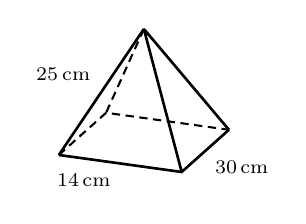
\begin{tikzpicture}[scale=0.80, every node/.style={font=\scriptsize, text=black}]
        \coordinate (P1) at (-1.30,-0.75);
        \coordinate (P2) at (0.65,-1.02);
        \coordinate (P3) at (1.40,-0.35);
        \coordinate (P4) at (-0.55,-0.08);
        \coordinate (V) at (0.05,1.25);
        \draw[black, line width=0.95pt] (P1) -- (P2) -- (P3) (V) -- (P1) (V) -- (P2) (V) -- (P3);
        \draw[black, line width=0.75pt, densely dashed] (P1) -- (P4) -- (P3) (V) -- (P4);
        \node[above left=0.5pt] at ($0.5*(V)+0.5*(P1)$) {$25\unit{cm}$};
        \node[below left=0pt] at ($0.5*(P1)+0.5*(P2)$) {$14\unit{cm}$};
        \node[below right=0pt] at ($0.5*(P2)+0.5*(P3)$) {$30\unit{cm}$};
      \end{tikzpicture}
    \end{center}
    $\bullet$ \textbf{ក.} មិនមែនពីរ៉ាមីតនិយ័តទេ ព្រោះបាតជា \blank{2.8cm}\\[3.5pt]
    $\bullet$ \textbf{ខ.} អាប៉ូតែមលើជ្រុង $14$: $d_1 = \sqrt{25^2 - 7^2} = \blank{1.3cm}\unit{cm}$\\[3.5pt]
    \hspace*{0.2cm}អាប៉ូតែមលើជ្រុង $30$: $d_2 = \sqrt{25^2 - 15^2} = \blank{1.3cm}\unit{cm}$\\[3.5pt]
    \hspace*{0.2cm}$S_l = (14\times\blank{0.9cm}) + (30\times\blank{0.9cm}) = \blank{1.4cm}\unit{cm}^2$\\[3.5pt]
    $\bullet$ \textbf{គ.} $S_t = S_l + (14\times 30) = \blank{1.2cm} + 420 = \blank{1.4cm}\unit{cm}^2$ ។
  \end{tcolorbox}
\end{minipage}

\vspace{7pt}
% --- E5 Evaluate: Composite Solid Ex #4 + Exit Check ---
\secbar{ផ្នែកទី៤ ៖ វាយតម្លៃ \enbf{---} សូលីតផ្សំលំហាត់ទី៤ \enbf{(}ទំ\enbf{.}២២៧\enbf{)} និង \enbf{Exit Check (E5)}}{ធ្វើដោយឯករាជ្យ \en{10 min}}

\noindent
\begin{minipage}[t]{10.3cm}\vspace{0pt}
  \begin{tcolorbox}[
    enhanced, sharp corners, colback=white, colframe=black, equal height group=rowE5,
    boxrule=0.85pt, boxsep=3pt, top=5pt, bottom=5pt, left=5.5pt, right=5.5pt
  ]
    \textbf{៤.ក លំហាត់ទី៤ ក, ខ (ទំ.២២៧)៖ សូលីតផ្សំ គូប + ពីរ៉ាមីតនិយ័ត}\\[3pt]
    \begin{minipage}[c]{6.4cm}\raggedright
      សូលីតខាងស្ដាំផ្គុំដោយគូបជ្រុង $10$ និងពីរ៉ាមីតចតុមុខនិយ័តដែលមានទ្រនុងខាង $13$៖\\[4pt]
      $1.$ \textbf{ក.} តើមុខ $ABCD$ ជាមុខខាងក្រៅនៃសូលីតនេះឬទេ?\\
      \hspace*{0.15cm}\chkbox\ មែន \hspace{0.3cm} \chkbox\ មិនមែន (ព្រោះនៅខាងក្នុង!)\\[4pt]
      $2.$ \textbf{ខ.} ចំនួនមុខសរុបនៃសូលីតផ្សំ៖\\
      \hspace*{0.15cm}$\blank{0.8cm}\text{ (គូប)} + \blank{0.8cm}\text{ (ពីរ៉ាមីត)} = \blank{0.9cm}$ មុខ ។
    \end{minipage}%
    \hfill
    \begin{minipage}[c]{3.3cm}
      \centering
      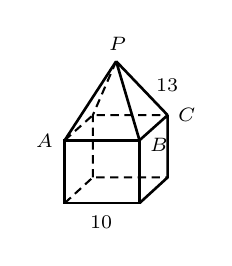
\begin{tikzpicture}[scale=0.76, every node/.style={font=\scriptsize, text=black}]
        \draw[black, line width=0.95pt] (-0.80,-0.95) rectangle (0.45,0.10);
        \draw[black, line width=0.95pt] (0.45,-0.95) -- (0.92,-0.52) -- (0.92,0.52) (0.45,0.10) -- (0.92,0.52);
        \draw[black, line width=0.75pt, densely dashed] (-0.80,0.10) -- (-0.33,0.52) -- (0.92,0.52) (-0.80,-0.95) -- (-0.33,-0.52) -- (0.92,-0.52) (-0.33,-0.52) -- (-0.33,0.52);
        \coordinate (P) at (0.06,1.42);
        \draw[black, line width=0.95pt] (P) -- (-0.80,0.10) (P) -- (0.45,0.10) (P) -- (0.92,0.52);
        \draw[black, line width=0.75pt, densely dashed] (P) -- (-0.33,0.52);
        \node[above=0.5pt] at (P) {$P$};
        \node[left=0.5pt] at (-0.80,0.10) {$A$};
        \node[right=0.5pt] at (0.45,0.02) {$B$};
        \node[right=0.5pt] at (0.92,0.52) {$C$};
        \node[below=1pt] at (-0.18,-0.95) {$10$};
        \node[right=1pt] at (0.52,1.02) {$13$};
      \end{tikzpicture}
    \end{minipage}\\[5pt]
    $3.$ រកអាប៉ូតែមពីរ៉ាមីត៖ $d = \sqrt{13^2 - 5^2} = \blank{1.1cm} \Rightarrow S_{l,\text{ពីរ៉ាមីត}} = \blank{1.4cm}$ ។
  \end{tcolorbox}
\end{minipage}%
\hfill
\begin{minipage}[t]{8.5cm}\vspace{0pt}
  \begin{tcolorbox}[
    enhanced, sharp corners, colback=white, colframe=black, equal height group=rowE5,
    boxrule=0.85pt, boxsep=3pt, top=5pt, bottom=5pt, left=5.5pt, right=5.5pt
  ]\raggedright
    \textbf{៤.ខ សំណួរត្រួតពិនិត្យរហ័ស (\en{Exit Check})៖}\\
    គូសវង់ជុំវិញអក្សរនៃចម្លើយត្រឹមត្រូវតែមួយគត់៖\\[5.5pt]
    \textbf{សំណួរទី១៖} រូបមន្តផ្ទៃក្រឡាទាំងអស់នៃពីរ៉ាមីតគឺ៖\\[2pt]
    \hspace*{0.15cm}\textbf{ក.} $S_t = S_l + 2B$ \hspace{0.3cm} \textbf{ខ.} $S_t = S_l + B$ \hspace{0.3cm} \textbf{គ.} $S_t = 2S_l + B$\\[6.5pt]
    \textbf{សំណួរទី២ (បេសកកម្ម \en{E1})៖} ពីរ៉ាមីតចតុមុខនិយ័តមានជ្រុងបាត $12$ និងទ្រនុងខាង $10$ មានអាប៉ូតែម $d$ ស្មើនឹង៖\\[2pt]
    \hspace*{0.15cm}\textbf{ក.} $10$ \hspace{0.75cm} \textbf{ខ.} $6$ \hspace{0.75cm} \textbf{គ.} $8$\\[6.5pt]
    \textbf{សំណួរទី៣៖} សូលីតផ្សំរវាងគូបមួយ និងពីរ៉ាមីតចតុមុខមួយដែលបិទពីលើមុខគូបពេញ មានមុខខាងក្រៅសរុបចំនួន៖\\[2pt]
    \hspace*{0.15cm}\textbf{ក.} $9$ មុខ \hspace{0.55cm} \textbf{ខ.} $10$ មុខ \hspace{0.55cm} \textbf{គ.} $11$ មុខ
  \end{tcolorbox}
\end{minipage}

\vspace{7pt}
% --- Step 5 Homework Box ---
\secbar{ផ្នែកទី៥ ៖ កិច្ចការផ្ទះ និងបណ្ដាំផ្ញើ \enbf{(}ទំព័រ ២២៧\enbf{--}២២៨ លំហាត់ទី៤គ និងទី១០ខ\enbf{,}គ\enbf{)}}{ធ្វើនៅផ្ទះក្នុងសៀវភៅសរសេរ}

\begin{tcolorbox}[
  enhanced, sharp corners, colback=panelgray, colframe=black,
  boxrule=0.85pt, boxsep=3.5pt, top=5pt, bottom=5pt, left=6pt, right=6pt
]
  \begin{minipage}[c]{14.0cm}\raggedright
    $1.$ \textbf{លំហាត់ទី៤គ (ទំ.២២៧)៖} បន្តពីផ្នែកទី៤ខាងលើ ចូរគណនាផ្ទៃក្រឡាសរុបនៃសូលីតផ្សំ ($S_{\text{សរុប}} = S_{l,\text{ពីរ៉ាមីត}} + 5\times 10^2$) ។\\[3pt]
    $2.$ \textbf{លំហាត់ទី១០ ខ, គ (ទំ.២២៨)៖} ពីរ៉ាមីតចតុមុខ $V\text{-}ABCD$ មានបាតជាការេជ្រុង $10\unit{cm}$ ($OY=OZ=5\unit{cm}$, ដូចរូបស្ដាំ) និងកម្ពស់ $VO=12\unit{cm}$ ។ គណនា៖ \textbf{ខ.} ផ្ទៃក្រឡាខាង $S_l$ \; \textbf{គ.} ផ្ទៃក្រឡាសរុប $S_t$ ។\\[3pt]
    $3.$ \textbf{អានមេរៀនបន្ទាប់៖} ១៧.១ ផ្ទៃក្រឡាខាងនិងផ្ទៃក្រឡាទាំងអស់នៃកោន (ទំ.២២០\,\en{--}\,២២២) ។
  \end{minipage}%
  \hfill
  \begin{minipage}[c]{4.0cm}
    \centering
    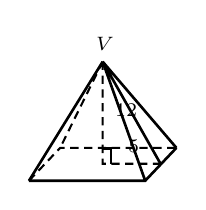
\begin{tikzpicture}[scale=0.72, every node/.style={font=\scriptsize, text=black}]
      \coordinate (A) at (-1.40,-0.80);
      \coordinate (B) at (0.65,-0.80);
      \coordinate (C) at (1.20,-0.22);
      \coordinate (D) at (-0.85,-0.22);
      \coordinate (O) at (-0.10,-0.50);
      \coordinate (V) at (-0.10,1.30);
      \coordinate (Z) at (0.92,-0.50);
      \draw[black, line width=0.95pt] (A) -- (B) -- (C) (V) -- (A) (V) -- (B) (V) -- (C) (V) -- (Z);
      \draw[black, line width=0.75pt, densely dashed] (A) -- (D) -- (C) (V) -- (D) (V) -- (O) -- (Z);
      \rightbox[0.15]{V}{O}{Z}
      \node[above=0.5pt] at (V) {$V$};
      \node[right=1pt] at (-0.10,0.45) {$12$};
      \node[above=0.5pt] at (0.45,-0.50) {$5$};
    \end{tikzpicture}
  \end{minipage}
\end{tcolorbox}

\end{document}
